% Chapter 3

\chapter{Research Methodology} % Main chapter title

\label{Chapter3} % For referencing the chapter elsewhere, use \ref{Chapter3} 

\lhead{Chapter 3. \emph{Research Methodology}} % This is for the header on each page - perhaps a shortened title

%----------------------------------------------------------------------------------------
In this work,  the aodv protocol slightly enhanced for making this protocol to detect blackhole node. Have to add some extra code in the header file of the protocol. The routing table and receive request is modified for this system build.



\section{Introduction}

Blackhole node is detected by this system. and information about detection is sent in the terminal. Admin may block this particular node from this network.\\
AODV protocol depends on some header files. we should have configured those files also.
%Figure   
\begin{figure}[htbp]
	\centering
	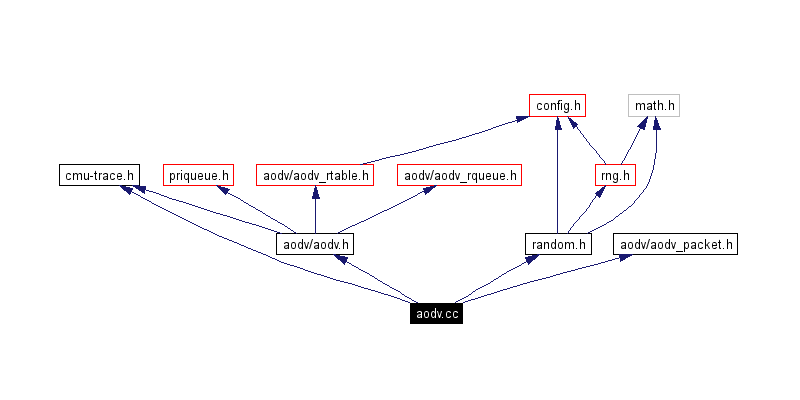
\includegraphics[scale=0.4]{aodv1}
	\rule{35em}{0.5pt}
	\caption[Dependencies of aodv.cc]{Dependencies of aodv.cc}
	\label{Dependencies of aodv.cc}
\end{figure}
\pagebreak
In this project, the nature of the blackhole attack is used to detect the blackhole node.
The main purpose of this work to detect malicious node in a crowded road where the blackhole mislead us in a wrong road where there is a barricade or the road is blocked.

%Figure   
\begin{figure}[htbp]
	\centering
	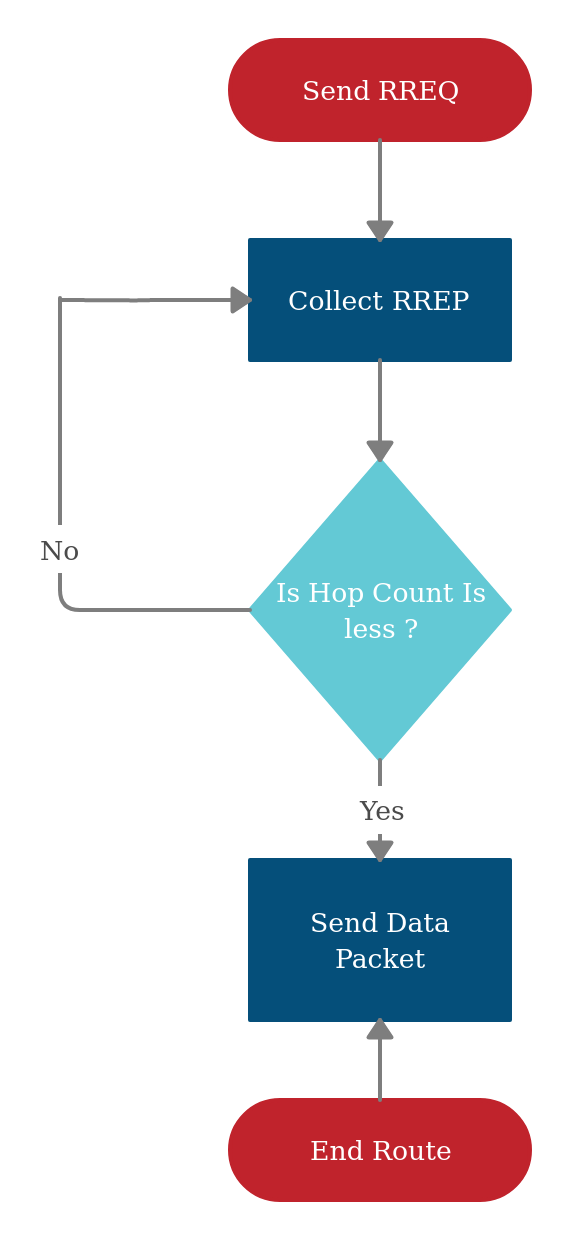
\includegraphics[scale=0.2]{algorithm}
	\rule{35em}{0.5pt}
	\caption[Algorithm Of Work]{Work Flow}
	\label{flow}
\end{figure}

\section{Research Subject and Instrumentation}

First of all, A VANET is created using OSM. This file is used as a source of the TCL file of the network that takes up from the ns2 package. The TCL file is used to mark a node as malicious. After that, aodv.cc and aodv.h is edited to implement the main detection algorithm. \\\\
In Blacklist table, each node will check its table to identify
whether the packet is coming from the malicious node. If this is
true, it will discard the packet. Also when any node identifies
the malicious node, it will send alarm packets to the entire
network about the malicious behaviors of the node thereby
removing the node from the routing table and adding it in the
blacklist table.

\subsection{SUMO}
Sumo is an application to generate a vanet network. we use two tools of sumo application and they are \\
1. osm web wizerd\\
2.trace exporter\\\\
osmWebWizerd is used to get real-time data from the map and generate a network scenario. After that, we use trace exporter to convert this scenario to a trace file.


\subsection{NS2}
It is a discrete-time simulator. The designed protocol can be applied in it. NS2 is a mostly used open-source simulation application. \\
Though there is a new version of ns named ns3, the older version is used because of having efficient knowledge in ns2.
\subsection{Tracegraph}
The trace file is analyzed with tracegraph. Two trace file (with malicious node, without malicious node) is created, observing both files and see the difference in between them. Three parameter is used in this project.

\section{Data Collection Procedure}
Auto-generated traffic mobility data is created with sumo application.
It auto-generates in real-world locations and has information about authentic data. It uses python package as it's design.

%Figure   
\begin{figure}[htbp]
	\centering
	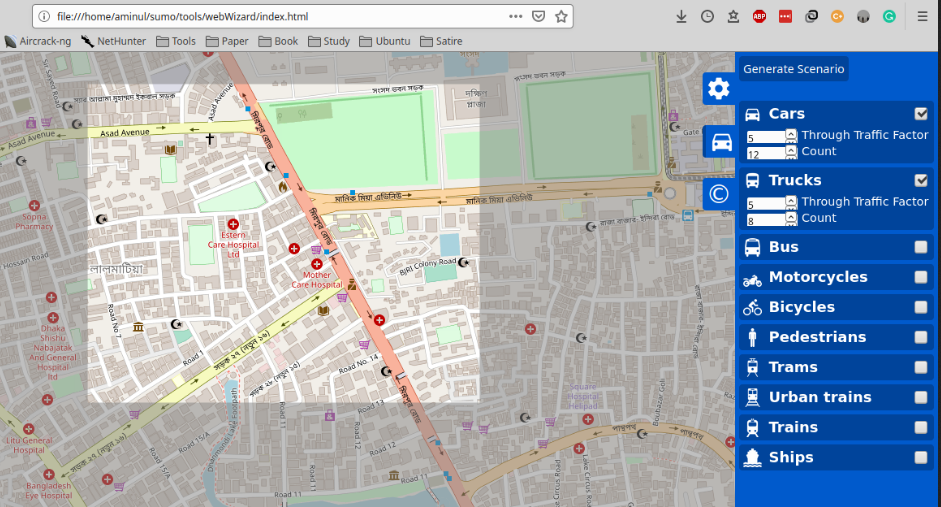
\includegraphics[scale=0.5]{sumo}
	\rule{35em}{0.5pt}
	\caption[Data Collection]{Data Collection}
	\label{Data Collection}
\end{figure}

\pagebreak
\section{Implementation Requirements}
Requirements of this project are \\
1. Basic command of the Linux operating system.\\
2. Clear idea about network and routing.\\
3. NS2 is the simulation application. Have to have an idea about build and change routing code of it.\\
4. analyzation of simulation performed using tracegraph. Basic parameter of a network like throughput, jitter cumulative sum, etc.\\
5. All ns2 code is written in C++. Have to have the ability to understand those code.